% % % % % % % % % % % % % % % % % % % % % % % % % % % % % % % % % % % % % % % % 
% Formelsammlung von LaTeX4EI									
%
% @encode: 	UTF-8, tabwidth = 4, newline = LF
% @author:	Emanuel Regnath
% @date:		
%
% % % % % % % % % % % % % % % % % % % % % % % % % % % % % % % % % % % % % % % % 


%---------------------------------------%
%			P R E A M B L E				%
%~~~~~~~~~~~~~~~~~~~~~~~~~~~~~~~~~~~~~~~%

% Document Class ===============================================================
\documentclass[fs, footer]{latex4ei}

\sisetup{per-mode = fraction}

%---------------------------------------%
%			Nachrichtentechnik 			%
%~~~~~~~~~~~~~~~~~~~~~~~~~~~~~~~~~~~~~~~%

% DOCUMENT_BEGIN ===============================================================
\begin{document}

% Split in 4 Columns ===========================================================
\begin{multicols*}{4}

% TITLE ========================================================================
\fstitle{Nachrichtentechnik}


% Shanon: A Mathematical Theory of Communication 1948
\sectionbox{
\Fbox{Quelle} $\ra$ \Fbox{Sender} $\ra$ \Fbox{Kanal} $\ra$ \Fbox{Empfänger} $\ra$ \Fbox{Senke}\\
\\
\\
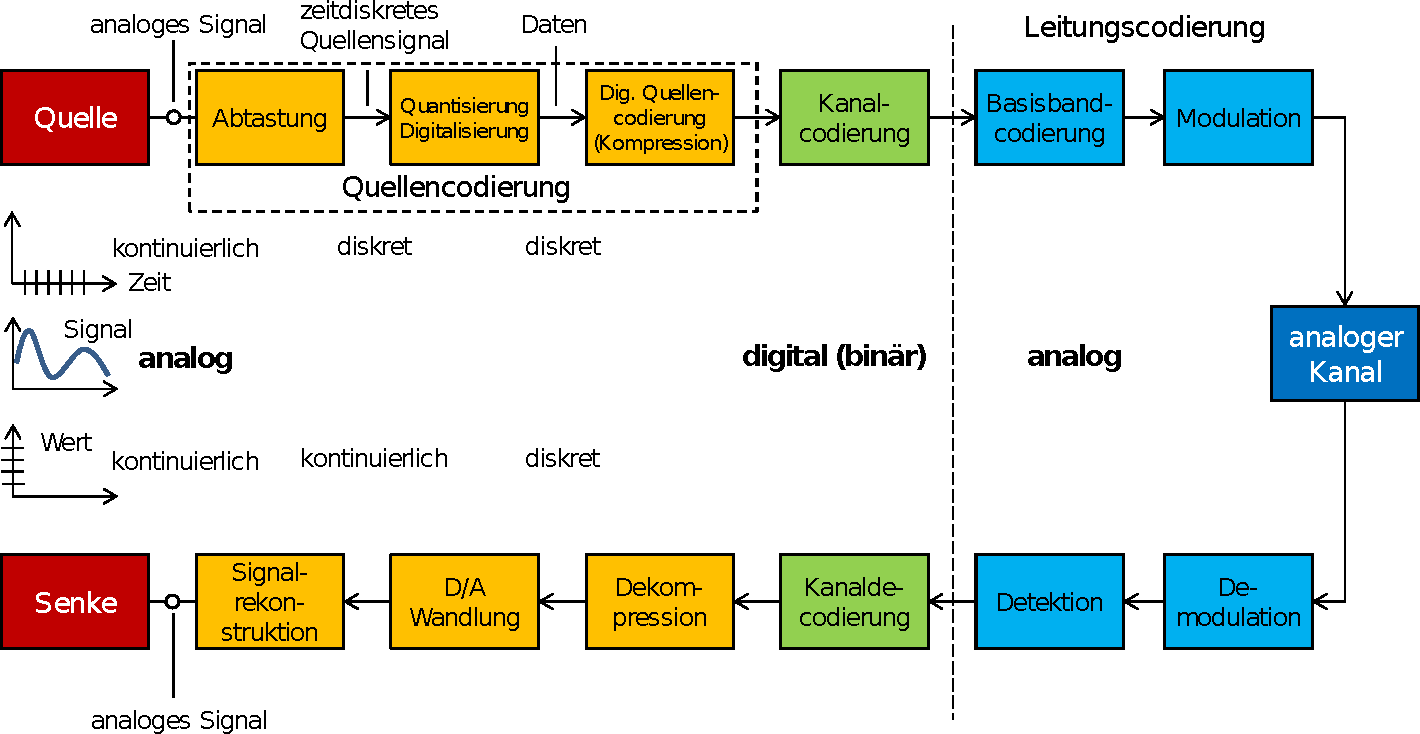
\includegraphics[width = \columnwidth]{./img/transmission.pdf}
}

% SECTION ====================================================================================
\section{Signale}
% ============================================================================================
	\subsection{Arten von Signalen}
	\begin{description}
		\item[deterministisch:] durch Funktionen beschreibbar, enthalten kein Nachricht.
		\item[stochastisch:] zufälliger Verlauf, überträgt Information
	\end{description}
	
	
	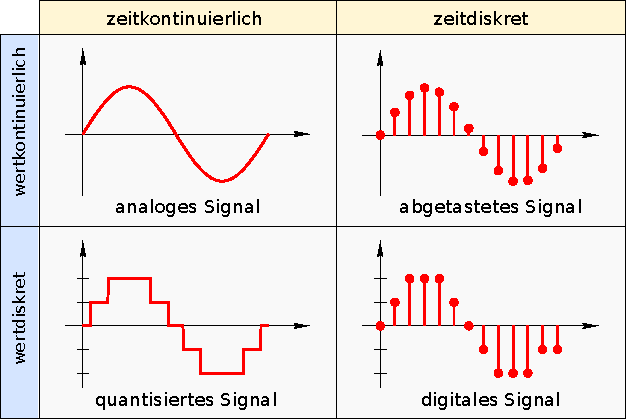
\includegraphics[width = \columnwidth]{./img/signals.pdf}



	\subsection{Frequenztransformationen}
	Wichtige Fouriertransformationen:\\
	\begin{tabular}{rl|rl}
		$f(t)$ & \qquad $F(\omega)$ & $f(t)$ & \qquad $F(\omega)$\\		%Graph mit zwei Farben?
		$1$ & \!\!\!\!\!\!\!\!\!\! $\laplace 2\pi \delta(\omega)$ & $|t^n|$ & \!\!\!\!\!\!\!\!\!\! $\laplace \frac{2n!}{(\i \omega)^{n+1}}$\\
		$t^n$ & \!\!\!\!\!\!\!\!\!\! $\laplace 2\pi \i^n \delta^{(n)}(\omega)$ & $\frac{t^{n-1}}{(n-1)!} e^{-at} u(t)$ & \!\!\!\!\!\!\!\!\!\! $\laplace \frac{1}{(a+\i \omega)^n}$\\[0.5em]
		$\heavi(t)$ & \!\!\!\!\!\!\!\!\!\! $\laplace \frac{1}{\i \omega} + \pi \delta(\omega)$ & $\delta(t-t_0)$ & \!\!\!\!\!\!\!\!\!\! $\laplace e^{-\i \omega t_0}$
	\end{tabular}

	Bei periodischen Signalen: Fourierreihen!\\
	$x(t),y(t)$ sind orthogonal, falls $\int\limits_{-\infty}^\infty x(t)y(t) = 0$


	\subsection{Sonstiges}
	Autokorrelation $r_{\textsf{V}}(\tau) \FT S_{\textsf{V}}(f)$ Leistungsdichtespektrum
	
	
	\subsection{White Gausian Noise (WGN)}
	Weiß, da alle Frequenzen enthalten sind.
	Autokorrelation = 0
	


% SECTION ====================================================================================
\section{Abtastung von Signalen}
% ============================================================================================
\sectionbox{
\subsection*{Abtasttheorem}
Signal $x(t)$, Abtastfunktion $s(t) = \sum \delta(t-nT_s)$, Tiefpassfilter $h_r(t)$\\
\\
\begin{tabular*}{\columnwidth}{@{\extracolsep\fill}lll@{}}
	Vorgang & Zeitbereich & Frequenzbereich\\
	Abtasten: & $x_s(t) = s(t) \cdot x(t)$ & $X_s(\omega) = S(\omega) * X(\omega)$\\
	Rekonstr. & $x_r(t) = h_r(t) * x_s(t)$ & $X_r(\omega) = H_r(\omega) \cdot X_s(\omega)$\\
\end{tabular*}

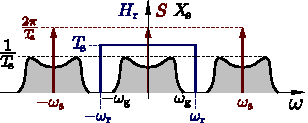
\includegraphics[scale = 1.3]{./img/sampletheorem.pdf}\\

Bandbreite $\omega_g$, Abtastfrequenz $\omega_s$\\
\\
\boxed{ \omega_s = \frac{2 \pi}{T_s} \ge 2 \omega_g } \qquad \boxed{ \omega_g \le \omega_r \le \omega_s - \omega_g }

Abtastoperator: $\mathbb A\{x(t)\} = x(t) \cdot T_A \sum \limits_{n = - \infty}^{\infty} \delta (t - n T_A)$ \\
Periodisierungsoperator: $\mathbb P \{ X(f) = X(f) * \sum \limits_{n = - \infty}^\infty \delta (f - \frac{n}{T_A})\}$
}

Faltungen:\\
	$\sinc\left(\frac{t}{T_A}\right) * \sinc\left(\frac{t}{T_A}\right) = T_A \sinc\left(\frac{t}{T_A}\right)$\\

Projektion: $\int\limits_{-\infty}^{\infty} x(t) \sinc\left( \frac{t- nT_A}{T_A}\right) \diff t = T_{\ir A} x(n T_A)$\\
$\int\limits_{-\infty}^{\infty} b_n(t) b_m(t) \diff t = \delta[m-n]$\\ 


Sample\&Hold: 



Interpolation $\rightleftarrows$ Dezimierung\\



% SECTION ====================================================================================
\section{Quantisierung und Digitalisierung}
% ============================================================================================

Quantisierung $\vec x_Q = \mathcal Q(\vec x)$\\
Bildet Vektoren $\vec x \in \R^N$ auf eine Menge $S$ ab mit $\abs{S} = M$\\
Man benötigt $m = \ceil{\log_2 M}$ bits um $\vec x_Q$ zu repräsentieren.\\
Intervall $I_i = [g_i, g_{i+1}]$ enthält Reprodwert $s_i$\\
Skalare Quantisierer: $N=1$ \qquad Vektor Quantisierer: $N > 1$\\


	\subsection{Lineare Quantisierung}
	Gleich große Quantisierungsintervalle

	Fehlerleistung $P_Q = \E[Q^2] = \int q(x)^2 f_{\X}(x) \diff x = \sum \int_{g_i}^{g_{i+1}} (s_i - x)^2 f_{\X}(x) \diff x$\\
	Bei gleichverteiltem Quantisierungsfehler: $P_Q = \frac{\Delta^2}{12}$\\
	$\SNR = \frac{P_S}{P_Q}$ \qquad $P_S = \E[X^2]$\\
	\\
	Optimales $\Delta = \frac{2 x_{\max}}{2^m}$ \qquad Reproduktionswerte $s_i = \frac{2i - M + 1}{2} \Delta$

	\subsection{Optimale skalare Quantisierung}
	\cookbox{Lloyd-Max-Algorithmus}{
		\item Wähle Startwerte für alle $s_i^{(0)}$
		\item Intervallgrenzen: $g_i^{(t+1)} = \frac{ s_i^{(t)} + s_{i-1}^{(t)} }{2}$  \qquad $i = 1, \ldots , M-1$
		\item Reprod. Werte: $s_i^{(t+1)} = \E[\X | \X \in I_i]$ \quad\ $i = 0, \ldots , M-1$
		\item Fehlerleistung $P_Q^{(t+1)} = \E[Q^2]$ mit $s_i^{(t+1)}$ und $g_i^{(t+1)}$
		\item Berechne relative Änderung $\delta^{(t)} = \frac{P_Q^{(t+1)}-P_Q^{(t)}}{P_Q^{(t)}}$
	}
		
			Mittlere Weglänge $\overline l = \sum \limits_{i= 0}^{n-1} p_i l_i$

	\subsection{Nichtlineare Quantisierung}
	A-law-Kennlinie (Europa) und $\mu$-law-Kennlinie (USA)\\
	$C(x) = \begin{cases} \frac{A}{1 + \ln(A)} \cdot \abs{x} \cdot \sgn(x) & 0 \le \abs{x} \le \frac{x_{\max}}{A} \\[1em]
	\frac{1 + \ln\left( \frac{A \cdot \abs{x}}{x_{\max}} \right)}{1 + \ln(A)} \cdot \abs{x} \cdot \sgn(x) & \text{sonst} \end{cases}$

	$A = 87.5 = \SI{24}{\decibel}$

	\subsection{Pulse Coded Modulation PCM}
	Abtastung + skalare Quantisierung\\
	
		\subsubsection{Differentielle PCM (DPCM)}
		Kann bei schnellen, großen Änderungen nicht mehr folgen.\\

		\subsubsection{Delta-Modulation}
		1-Bit-Quantisierung: $e_Q(nT_{\ir S}) = \pm \Delta$\\
		Kann den Wert nicht Konstant halten, Tiefpass am Empfänger nötig\\

		\subsubsection{Sigma-Delta-Modulator}
		$\sum$: Summe/Integral \qquad $\Delta$: 1-bit-Quantisierer


	\subsection{Informationsgehalt und Entropie}
	Info vom Symbol $s_i$: $I_i = - \log_2 \P(\X_Q = s_i) = -\log_2 p_i$\\ 
	Entropie von $\X_Q$: $H(\X_Q) = \E[I] = - \sum\limits_{i = 0}^{M-1} p_i \log_2 p_i$\\

	Die minimale mittlere Codewortlänge $\overline l \ge H(x_Q)$
% SECTION ====================================================================================
\section{Codierung}
% ============================================================================================
	Komprimierung: Falls Bitstrom nicht gleichverteilt und mit Gedchtnis\\
	Maximale Kompression: Bits gleichverteilt, ohne Gedächtnis\\

	\subsection{Kompression}
	Kleiner Verlust bei unkodierten Bitstrom. Großer Gewinn bei Kodierung.\\
	Bsp: Feste Blocklänge mit Statusbit am Anfang: Kodiert/Unkodiert\\
	
	\subsection{Digitale Quellencodierung (Kompression)}
	Arten von Kodierern:
	\begin{description}
		\item[Verteilung Bekannt:] Huffman Code, Morse, Arithmetic
		\item[Universal:] Lempel-Ziv (ZIP), PPM, BWT(bZip)
		\item[Transform:] Fouriertransformation (JPG,GIF,PNG,MP3)
	\end{description}
	%Kompression, Vektorquantisierung (verlustbehaftet) 

	\subsection{Kanalcodierung}
	Single-Parity-Check: 1 Bit pro 2 bit zusätzlich: XOR$(x_1,x_2)$\\
	Daraus ergibt sich eine Effizienz von $\frac{2}{3}$\\
	\\
	FEC: Forward Error Correction liefert Fehlererkennung und Korrektur.\\
	Beispiele: Paritätsbit, CRC, Reed-Solomon-Codes, LDPC,  Polar Codes
	
	% Paper Award IEEE: Polar Codes
	% Kanal lässt bestimmte Frequenzen durch: Luft hat bei 60GHz ein Minimum weil Wassermoleküle dagegen schwingen.



% SECTION ====================================================================================
\section{Basisbandübertragung}
% ============================================================================================
PAM: Puls-amplituden-modulations-verfahren\\
\\
	Wie wählt man $g(t)$?\\
	Ressourcen: Zeit, Bandbreite, Energie, (Raum)\\



	\subsection{Impulsformen}
	Rechteckimpuls: $g(t) = \rect\left(\frac{t}{T}\right)$\\
	Manchaster Impuls: Mittelwert Null, kein Gleichstrom\\
	$\cos^2$-Impuls: $g(t) = \cos^2\left(\frac{\pi t}{T}\right)$ für $\abs{t} < \frac{T}{2}$\\
	
	$\sinc$-Impuls: $g(t) = \sinc\left(\frac{t}{T}\right)$\\
	„Nyquist roll-off“-Impuls:\\
	Root-Raised-Cosine: Meist genutzer Filter (Wurzel-Nyquist)\\
	Gauß-Impuls: $g(t) = \exp\left[ -\pi\left( \frac{t}{\Delta t} \right) \right]$\\
	
	
	\subsection{Bandbreite}
	Absolut: Alle positiven Frequenzen\\
	B$_99$ Bandbreite: 90\% der Frequenzen\\
	B$_{\ir 6dB}$ Bandbreite: Bis Hälfte des Spektrums $G(f)$\\
	B$_{\ir 3dB}$ Bandbreite: Bis Hälfte der Leistung\\
	B$_N$\\
	\\
	Bandbreiteneffizienz $\eta = \frac{\text{Übertragungsrate}}{\text{Bandbreite}}$\\
	Beispiel GSM: $\eta = 0.88 \si{\kilo \bit/s \per \hertz}$, \quad LTE: $\eta = \frac{3 \si{Gbit/s}}{100 \si{\mega \hertz}} = 30$\\
	\\
	$E = \int\limits_{-\infty}^\infty g^2(t) \diff t = \int\limits_{-\infty}^\infty \abs{G(f)}^2 \diff f$\\
	Bandbreite: $B_0^2 = \frac{1}{E} \int\limits_{-\infty}^\infty f^2 \abs{G(f)}^2 \diff f$\\
	$T_D^2 = \frac{1}{E} \int\limits_{-\infty}^\infty t^2 \abs{g(t)}^2 \diff t$\\
	Unschärfe: $T_D \cdot B_0 \ge \frac{1}{4\pi}$\\
	Ein Signal kann nicht gleichzeitig hart Band- und Zeitbegrenzt sein! 


\sectionbox{
\subsection{Korrelation}
Ein Maß für die Ähnlichkeit zweier Signale $x(t), y(t)$ bei Verschiebung.\\
Korrelationskoeffizient $\rho_{xy} = \frac{E_{xy}}{\sqrt{E_x \cdot E_y}} = \frac{\varphi_{xy}(0)}{ \sqrt{\varphi_x(0) \cdot \varphi_y(0)}}$\\
\\
Es gilt: Korreliert $\rho = 1$, Orthogonal $\rho = 0$, Antipodisch $\rho = -1$\\
\\
\textbf{Kreuzkorrelationsfkt.} zwischen zueinander verschobenen Signalen:\\
	\emphbox{ $\displaystyle \varphi_{xy} (\tau) =  \varphi_{yx}(-\tau) = \int\limits_{-\infty}^{\infty} x(t) \cdot y(t+\tau) \diff t$ }
	Zusammenhang mit Faltung: $\varphi_{xy} (\tau) = x(-t) * y(t)|_{t = \tau}$\\
	\\
\textbf{Autokorrelationsfkt. AKF} ist Kreuzkorrelation mit sich selbst ($y = x$):\\
$\varphi_x (\tau) = \varphi_{xx}(\tau)$ \qquad (Zum Erkennen von Perioden).\\ 
\\
\textbf{Energiebeziehung:} $E_{x,y} = \rho_{x,y} \sqrt{E_x E_y}$ mit \\
$E_x = \int\limits_{- \infty}^{\infty} x(t)^2 \diff t = \int\limits_{- \infty}^{\infty} \Phi_x \diff f = \varphi_{xx}(0)$\\
\textbf{Leistungsdichtespektrum} $\Phi_x(f)$ ist definiert als $\varphi_x \FT \Phi(f)$\\

Periodische Signale: $\overline \varphi_{xy}(\tau) = \frac{1}{2T} \int_{-T}^{T} x(t) y(t+\tau) \diff t$\\
\textbf{Stochastische Signale:} $\varphi_{\X\Y}(\tau) = \E[\X(t) \cdot \Y(t+\tau)]$\\
$\rho_{\X,\Y} = \frac{\Cov[\X \Y]}{\sigma_{\X} \sigma_{\Y}}$\\
}




% SECTION ====================================================================================
\section{Analoger Übertragungskanal}
% ============================================================================================






\subsection{\textsc{AWGN} -- Additive White Gaussian Noise}
Weißes Rauschen $\textit{N}$\\
\begin{tabular}{ll}
PDF & $f_\textit{N}(n) = \frac{1}{\sqrt{2\pi \sigma}} e^{-\frac{n^2}{2\sigma^2}}$\\
LDS: & $\Phi_\textit{N} = \frac{N_0}{2}$ \qquad für $\omega < \SI{10}{\giga \hertz}$\\
AFK: & $\varphi_n = \frac{N_0}{2} \delta(\tau)$\\
Leistung & $_\textit{N} = \sigma^2 = B \cdot N_0$\\
\end{tabular}




% SECTION ====================================================================================
\section{Detektion im Rauschen}
% ============================================================================================
gewähltes Bit $\hat D_n$ eines tatsächlichen Bits $D_n = \eset{1,0}$\\
Ziel: $\P(\hat D_n \ne D_n)$ soll minimal sein.\\
Lösung: maximiere SNR zum Abtastzeitpunkt $nT$\\

	\subsection{Matched Filter}
Matched Filter: $h(t) = K \cdot \cxc g_s(T-t)$\\
Maximum SNR: $\frac{P_s}{P_N} = \frac{2E_s}{N_0}$\\

	\subsection{Fehlerwahrscheinlichkeit $P_b$}
	$P_b = \frac{1}{\sqrt{2 \pi}} \cdot \int_{z_0}^\infty e^{\frac{-z^2}{2}} \diff z = Q(z_0)$\\
	Substituiere $z_0$
	$P_b = Q(\sqrt{2 E_s / N_0}) = Q(\sqrt{SNR})$
	
	\subsection{Zeitdiskreter AWGN-Kanal}
	$\sigma^2 = \frac{\sigma_\textit{N}^2}{A^2} = \frac{N_0}{2 E_s} = \frac{1}{SNR}$\\
	
	\subsection{Unabhängiges (unkorreliertes) Rauschen}
	Falls die erste Nyquistbedingung erfüllt und maximale SNR: \\ $\Ra$ Die Folge abgetasteter Rauschanteile ist unabhängig!


% Ende der Spalten
\end{multicols*}

% Dokumentende
% ======================================================================
\end{document}

% ToDos:

